\documentclass[12pt]{article}
%\usepackage[utf8]{inputenc}
\usepackage{amssymb,amsmath,graphicx,url,fullpage,amsfonts,verbatim,natbib}
\usepackage[small,bf]{caption}

% add bib to ToC
\usepackage{tocbibind}

\newcommand{\tatonnement}{t\^atonnement}

\input defs.tex

\title{Computing Market Equilibria via Convex Optimization}
\author{A.J. Friend \and Stephen Boyd}
\date{\today}

\begin{document}

\maketitle

\begin{abstract}

We consider the pure exchange market equilibrium problem of finding prices such
that the market clears, \ie, demand does not exceed supply. This is a classic
problem in economics, and has been discussed recently in the literature from a
computational complexity perspective. Indeed, depending on the utility
functions of the agents in the market, finding equilibrium prices can be
NP-hard. This paper will focus on the numerical computation of equilibria for a
subset of markets whose equilibrium problem can be cast as a convex program.
Recent advances in exponential cone solvers allow us to solve these problems as
conic programs. We will also introduce algorithms which scale to huge markets
and can be computed in a distributed fashion. We report numerical results for
huge random markets.

\end{abstract}

\newpage
\tableofcontents
\newpage

%todo santiago's stuff

\section{Introduction}
\subsection{Background}

We will consider exchange market equilibrium problems first introduced by
Walras in his in ``Elements of Pure Economics'' \cite{walras1896elements}.
Walras considers a market with agents trading goods at prescribed prices to
maximize their own utility functions. The market equilibrium problem is that of
finding prices for the goods such that the total demand of the agents does not
exceed the total amount of each good supplied by the agents for trade.

In full generality, Walras' model includes \emph{production}, \ie, processes by
which existing goods can be consumed to produce new goods which may enter the
market. We restrict this paper to the pure exchange market, which allows for
trading of existing goods, but not production.

Walras suggested his natural \emph{\tatonnement{}} price adjustment scheme as a
means of computing equilibrium prices. However, the convergence of
\tatonnement{} and conditions for existence of equilibrium prices remained an
open problems for many years.

The Nobel Laureates Arrow and Debreu were the first to show that equilibrium
prices exist under mild conditions on the utility functions of agents
\cite{arrow1954existence}. However, these proofs relied on fixed-point theorems
\cite[see][]{border1989fixed}
and were initially non-constructive.
As such, they offered no practical means by which to compute these equilibria. 
However, Scarf and others 
\cite{scarf1967approximation,scarf1973computation,
scarf1982computation,eaves1972homotopies} were able to extend the fixed-point
ideas to produce path-following algorithms to compute equilibrium prices.
Unforunately, however, these algorithms had exponential worst-case running times.

Smale \cite{smale1976exchange,smale1976convergent} developed algorithms based
on Newton's method, but with no polynomial running time guarantees.

This paper will investigate formulations of the market equilibrium
problem as convex optimization problems \cite{BoV:04},
which were rediscovered by Jain \cite{jain2007polynomial}.
This focus will restrict the types of markets we can
consider, but the convex optimization framework will allow us to solve
these problems efficiently and at scale.
The original convex
formulations for linear utility functions
were stated by Nenakov
and Primak \cite{nenakov1983algorithm}. Jain's convex formulation was later
extended by Chen, Ye, and Zhang \cite{chen2007note, chen2010equilibrium} to
include some non-homogeneous utility functions.

Eisenberg and Gale \cite{eisenberg1959consensus, gale1960theory,
eisenberg1961aggregation} gave a convex program for a special case of Walras'
model which was first introduced by Fisher \cite[see][]{brainard2000compute}.
The Fisher model consists of agents purchasing goods instead of trading.
The convex formulation of this special case will allow us to handle a larger
family of utility functions.

While there are huge bodies of work across several disciplines covering the
economic interpretations, formulations, computational complexity, and
mathematical properties of these market equilibrium problems, our focus in
this paper is on developing efficient computational techniques to solve
numerical instances of the given problems.
We provide two algorithmic approaches to the convex formulations
of these problems. The first is to capitalize on recently
developed exponential cone solvers \cite{scs} to provide a centralized
algorithm, easily solved with a convex modeling language, such as \cite{cvxpy,
cvx}. The second approach is to use the \emph{alternating direction method of
multipliers} (ADMM) \cite{boyd2011distributed} to produce a distributed and
scalable algorithm, allowing us to tackle huge problems.

\subsection{Outline}

In \S\ref{sec:defs}, we define two different \emph{market equilibrium problems}
(MEP) for the exchange and Fisher markets. The MEPs are defined by describing
the \emph{utility maximization problems} (UMP) of the agents in these markets,
and requiring that the solutions to the UMPs satisfy an equilibrium condition.

In \S\ref{sec:convex_form}, we convert the exchange and Fisher MEPs into two
different optimization \emph{formulations} which provide convex programs when
the utility functions satisfy certain properties (\S\ref{sec:util_funcs}). We
will refer to these specifically as the exchange and Fisher \emph{formulations}
to emphasize that a single \emph{problem} may be solvable using either
\emph{formulation}.

An exchange MEP must always be solved using the exchange formulation. However,
depending on the utility functions of the agents, Fisher MEPs can be solved
using the Fisher formulation, or by converting to an exchange problem and using
the exchange formulation. There are some Fisher MEPs which can only be solved
using the exchange formulation.

Once we have used one of the two formulations to state an MEP as a convex
optimization problem, we can write down the problem easily using a convex
modeling language and solve it with an appropriate centralized solver
(\S\ref{sec:centralized}). However, these methods will only scale up to
medium-sized problems. For large scale problems, we will provide a distributed
algorithm in \S\ref{sec:distributed}. Luckily, the two convex formulations are
sufficiently similar that we can solve either one with this single distributed
algorithm.

We provide examples and convergence results for large random markets in
\S\ref{sec:examples}.


\section{Problem definitions}
\label{sec:defs}

In this section, we give precise definitions for the market equilibrium
problems that we will be studying. We define the exchange model, which deals
with agents trading initial endowments of goods to maximize their own utility
functions. A special case of the exchange model is Fisher model, where agents
start with some initial wealth, which they use to purchase goods  from a
globally available store.

Throughout the rest of the paper, $\reals^n_+$ will denote the nonnegative
real $n$-vectors, $\reals^n_{++}$ will denote the positive real $n$-vectors,
and inequalities between two vectors of the same size, \eg, $x \leq y$,
will denote componentwise inequality. When it isn't ambiguous, $0$ may stand
in for a vector of any size whose elements are all zero.

\subsection{Utility function properties}

The convexity of the resulting optimization problems will depend on properties
of the utility functions of the agents in the market. To classify these
functions, we state some simple definitions.

A function $u: \reals^n_+ \to \reals_+$ is \emph{homothetic} if for any $\alpha
> 0$ we have that $u(x) \geq u(y)$ if and only if $u(\alpha x) \geq u(\alpha
y)$. The function is \emph{monotone} or \emph{nondecreasing} if $x \geq y$
implies that $u(x) \geq u(y)$. It is \emph{homogeneous} of degree $d$ if for
any $\alpha > 0$, $u(\alpha x) = \alpha^d u(x)$.

All the utility functions we consider in this paper will be concave and
nondecreasing.

\subsection{Exchange market}
\label{sec:exchange_def}

An \emph{exchange market} has $m$ agents and $n$ goods where agent $i$ has an
initial endowment of goods $b_i \in \reals_+^n$. Agent $i$ achieves utility
$u_i(x_i) \in \reals_+$ when he is allocated a bundle of goods $x_i \in
\reals^n_{+}$, that is, he is allocated amount $x_{ij}$ of good $j$.

Given prices $p \in \reals^n_{++}$ for the goods, agent $i$ will sell his
initial bundle of goods, $b_i$, and buy a bundle of goods $x_i$ to maximize his
utility. That is, agent $i$ solves the \emph{exchange utility maximization
problem} (exchange UMP)
\begin{equation}
\label{p-ump}
\begin{array}{ll}
\mbox{maximize} & u_i(x_i) \\
\mbox{subject to} & p^T x_i \leq p^T b_i \\
& x_i \geq 0,
\end{array}
\end{equation}
with optimization variable $x_i$. Note that for fixed prices, $p$, the exchange
UMP is a convex optimization problem.

When it won't be confused with the optimization variable, we will denote the
\emph{set} of solutions to the exchange UMP as $x^\star_i(p)$, and refer to it
as the \emph{demand} of agent $i$ at prices $p$.
Formally, $x_i^\star : \reals^n_{++} \to 2^{\reals^n_+}$ is a \emph{relation},
\emph{set-valued mapping}, or \emph{correspondence}. When the optimal bundle is
unique, we may think of the demand as a \emph{function}.
Many utilities will result in a unique bundle, however, the simple 
case of the linear utility admits a demand relation.

The \emph{exchange market equilibrium problem} (exchange MEP) is to find prices
$p$ and endowments $x_i$ such that the demand for goods in the market does not
exceed the supply provided by the initial agent endowments. The exchange model
is also referred to as the Walras model \cite{walras1896elements}, the pure
exchange model, or the Arrow-Debreu model.

We can write the exchange MEP as the feasibility problem
\begin{equation}
\label{p-mep}
\begin{array}{ll}
\mbox{find} & p, x_1, \ldots, x_m \\
\mbox{subject to} & x_i \in x_i^\star(p),\quad i = 1,\ldots, m \\
& \sum_{i=1}^m x_i \leq B,
\end{array}
\end{equation}
where $B = \sum_{i=1}^m b_i$ is the vector giving the total amount of each good
available for trade.

In this paper, we will only consider markets where each good is \emph{desired}
by at least one agent, and each good is \emph{provided} by at least one agent,
by way of being included in that agent's initial endowment. These restrictions
will allows us to exclude special cases requiring zero or infinite prices.


\paragraph{Tractability}

In general, however, the exchange MEP is not convex. The computational
tractability of the exchange MEP (and the forthcoming Fisher MEP) depends on
the utility functions of the agents in the market. For example, for general
concave and increasing utility functions, the exchange MEP is NP-hard
\cite{codenotti2006leontief}. We will restrict our consideration in this paper
to a subset of utility functions for which the exchange MEP can be modeled as a
convex program.

In \S\ref{sec:convex_form_exchange}, the exchange MEP~(\ref{p-mep}) is
reformulated as a problem amenable to convex optimization. The convexity of the
problem will depend on properties of the agents' utility functions. The
admissible functions will include linear, constant elasticity of substitution
(CES), Cobb-Douglas, and a few other utilities. A full description of these
functions will be given in \S\ref{sec:util_funcs}. The convex formulation given
in \S\ref{sec:convex_form_exchange} will be the basis for the algorithms which
we will outline in \S\ref{sec:algorithms}.


\subsection{Fisher market}

We will also consider the Fisher market, a special case of the exchange market,
where agents have an initial amount of wealth (instead of an initial endowment
of goods) to purchase goods from a store of some amount of globally available
goods.

A \emph{Fisher market} has $m$ agents and $n$ goods where agent $i$ has an
initial amount of money, or wealth, $w_i \in \reals_{++}$. The total amount of
good $j$ available for purchase in the market is given by $B_j \in
\reals_{++}$.

Given good prices $p \in \reals^n_{++}$, agent $i$ uses his initial wealth
$w_i$ to buy a bundle of goods $x_i$ to maximize his utility $u_i$. That is,
agent $i$ solves the \emph{Fisher~UMP}
\begin{equation}
\label{p-fisher-ump}
\begin{array}{ll}
\mbox{maximize} & u_i(x_i) \\
\mbox{subject to} & p^T x_i \leq w_i \\
& x_i \geq 0.
\end{array}
\end{equation}
Note that the only difference between problem (\ref{p-ump}) and
(\ref{p-fisher-ump}) is that we have replaced $p^T b_i$ with $w_i$.

We will again use $x^\star_i(p)$ to denote the demand relation for agent $i$,
\ie, the set of solutions to the Fisher UMP~(\ref{p-fisher-ump}).

The \emph{Fisher MEP} is then identical to problem (\ref{p-mep}), except that
we use  the Fisher definitions for $x^\star_i(p)$ and $B$.


\paragraph{Fisher is a special case of Arrow-Debreu}

We can cast any Fisher equilibrium problem as an exchange market problem using
the following transformation.

Let $w_i$ be the wealth of agent $i$ and $B$ be the total amount of goods in
the Fisher system. Let $W = \sum_{i=1}^m w_i$ be the total wealth in the Fisher
market. To form the exchange market corresponding to the Fisher system, assign
an initial bundle of goods $b_i = B w_i/W$ to agent $i$. Since the scaling of
$p$ in the exchange problem is arbitrary, this gives the correct proportion of
wealth to each agent with the correct total amount of goods in the market.


\paragraph{Tractability}

As the Fisher problem is a special case of the exchange problem, if the agents'
utilities are compatible with the exchange formulation to be given in
\S\ref{sec:convex_form_exchange} we can transform the Fisher MEP to the
corresponding exchange problem to be solved using that formulation.

However, the Fisher problem will also admit a different convex model (to be
given in \S\ref{sec:convex_form_fisher}) which will extend the class of
compatible utility functions to those which are homogeneous of degree 1.
%todo reference for extension to homothetic
In particular, the Fisher MEP with
Leontief utility functions will be tractable as a convex problem, while the
exchange MEP with Leonteif utilities is NP-hard. The compatible utility
functions will be covered more completely in \S\ref{sec:util_funcs}.

Summarizing, a Fisher market with compatible utility functions can be solved
using the convex formulation in \S\ref{sec:convex_form_exchange}. If the Fisher
utilities are concave, nondecreasing, and homogeneous of degree 1, then we can
use the Fisher formulation of \S\ref{sec:convex_form_fisher}.


\section{Convex optimization formulations}
\label{sec:convex_form}
In this section, we cover the convex formulations which can be used to cast
the Fisher and exchange market equilibrium problems as convex programs.

\subsection{Exchange}
\label{sec:convex_form_exchange}

To avoid cases where we must consider prices which are zero or infinite,
throughout this paper, we will only consider markets where each good is desired
by at least one agent, and each good is provided by at least one agent. Under
this assumption, we can follow the formulations given in
\cite{jain2007polynomial, chen2007note, nenakov1983algorithm}, which show that
the optimality conditions for the exchange MEP (\ref{p-mep}) are equivalent to
the conditions
\begin{equation}
\begin{array}{ll}
& \nabla u_i(x_i)^T x_i \geq  \nabla_j u_i(x_i) \sum_k b_{ik} \frac{p_k}{p_j}\\
& \sum_i x_{ij} \leq \sum_i b_{ij}\\
& x_{ij} \geq 0,\ p_j \geq 0,
\end{array}
\label{p-exchange-gp}
\end{equation}
for all indices $i=1,\ldots,m,\ j=1,\ldots,n$, where $\nabla u_i(x_i)$
is any subgradient of $u_i$ at point $x_i$. That is, the optimality
conditions hold if there exist some subgradients for which (\ref{p-exchange-gp})
holds.
For a proof of this equivalence, see Appendix~\ref{sec:exchange_proof}.

Problem (\ref{p-exchange-gp}) is not yet in the best form to admit useful
convex programs, so we will apply some transformations to the problem.
Specifically, let $p_j = \exp(\phi_j)$, and take the logarithm of the first set
of constraints. We will refer to $\phi$ as the \emph{log-prices}.

We obtain the equivalent optimization problem
\begin{equation}
\label{p-exchange}
\begin{array}{ll}
\mbox{find} & x, \phi \\
\mbox{subject to} & \log(\nabla u_i(x_i)^T x_i) - \log(\nabla_j u_i(x_i)) + \phi_j 
\geq \log(\sum_k b_{ik} e^{\phi_k})\\
& \sum_i x_{ij} \leq \sum_i b_{ij}\\
& x_{ij} \geq 0,
\end{array}
\end{equation}
where the indices are again taken over all $i=1,\ldots,m,\ j=1,\ldots,n$.

Note that the optimization problem is convex if all the utility functions
in the market are such that the term
\begin{equation}
\label{e-util-constraint}
\log(\nabla u_i(x_i)^T x_i) - \log(\nabla_j u_i(x_i))
\end{equation}
is concave for all $i$ and $j$.
We will refer to (\ref{p-exchange}) as the \emph{exchange formulation}.

Note that the first constraint in (\ref{p-exchange}) only needs to be
explicitly formed when $\nabla_j u_i(x_i) > 0$; this derivative will be zero,
for example, if an agent has no interest in good $j$. Similarly, we only need
to include terms in the sum inside $\log(\sum_k b_{ik} e^{\phi_k})$ when
$b_{ik} > 0$. These ideas will be used later when we exploit sparsity to solve
these problems efficiently.

\subsection{Fisher}
\label{sec:convex_form_fisher}

When the utility functions are concave and homogeneous of degree 1,
the Fisher MEP can by solved by the convex program
\begin{equation}
\label{p-fisher}
\begin{array}{ll}
\mbox{maximize} & \sum_{i=1}^m w_i \log u_i(x_i) \\
\mbox{subject to} & \sum_{i=1}^m x_i \leq B\\
& x_i \geq 0\quad i=1,\ldots,m,
\end{array}
\end{equation}
originally given by \cite{eisenberg1959consensus, gale1960theory,
eisenberg1961aggregation}. For a proof, see \cite[\S6.2]{nisan2007algorithmic}.
We will refer to (\ref{p-fisher}) as the \emph{Fisher formulation}.

The objective in this convex program is sometimes referred to as a
\emph{weighted aggregate utility}, where the weights are given by the amount of
wealth $w_i$ possessed by agent $i$. Note that only allocations $x_i$ appear as
variables in the optimization problem. The equilibrium prices can be recovered
as dual variables.

\section{Utility functions}
\label{sec:util_funcs}

In this section, we'll describe various families of utility functions
and state whether they fit into the convex programming frameworks
for the exchange (\ref{p-exchange}) or Fisher (\ref{p-fisher}) formulations.
It will also
be valuable to note how the expressions associated
with the utility functions may be expressed in a disciplined
convex programming framework \cite{GBY:06,Grant2004,cvx,cvxpy}.


\subsection{Linear}

Linear utility functions have the form
\[
u(x) = a^T x.
\]

The utility is compatible with the exchange problem~(\ref{p-exchange}),
since
\[
\log(\nabla u(x)^T x) - \log(\nabla_j u(x))  = \log(a^T x) - \log(a_j)
\]
is concave.

This utility is compatible with the Fisher problem~(\ref{p-fisher}), as it is
homogeneous of degree 1.


\subsection{Constant elasticity of substitution}
Constant elasticity of substitution (CES) functions have the form
\[
u(x) = \left(\sum_{j=1}^n a_j x_j^\rho \right)^{1/\rho}.
\]
For $-\infty < \rho \leq 1, \rho \neq 0$, the utility is a concave and
increasing function.

It is useful to note that when $\rho = 1$, we have the linear utility function.
As $\rho$ approaches $0$ and $-\infty$ we recover the Cobb-Douglas and Leonteif
utility functions in the limit. %todo check which one is which

This utility is compatible with Fisher convex formulation, as it is concave and
homogeneous of degree 1.

For the exchange formulation, some algebra shows that 
\begin{align*}
\log(\nabla u(x)^T x) - \log(\nabla_j u(x)) =
\log\left(\sum_{k=1}^n a_k x_k^\rho \right) - \log a_j + (1-\rho) \log x_j,
\end{align*}
which is only concave when $0 < \rho \leq 1$.

Although we won't cover it in this paper, Codenotti and McCune
\cite{codenotti2005marketCES} were able to provide a convex formulation which
accommodated CES functions with $-1 \leq \rho < 0$.

\subsection{Cobb-Douglas}
The Cobb-Douglas utility has the form
\[
u(x) = \prod_{j=1}^{n} x_j^{a_j},
\]
where $\sum_j a_j = 1$.


The utility is concave and homogeneous, so it is compatible with the Fisher
convex formulation.

For the exchange formulation, we have that
\begin{align*}
\log(\nabla u(x)^T x) - \log(\nabla_j u(x)) =
\log x_j - \log a_j,
\end{align*}
which is indeed concave, so the utility is also compatible with
formulation~(\ref{p-exchange}).

\subsection{Piecewise-linear concave and Leontief}
Piecewise-linear concave functions have the form
\[
u(x) = \min_k\lbrace a^{kT}x \rbrace,\quad a^k \geq 0.
\]

A special case, the Leontief utility,
\[
u(x) = \min_j a_j x_j,
\]
with $a_j \geq 0$ for each $j$,  comes from the economics literature. 

These utilities are compatible with the Fisher formulation, as they are
homogeneous and concave. However, they are not compatible with the exchange
formulation, as the expression~(\ref{e-util-constraint}) is not concave. In
fact, the Leonteif utility admits multiple disconnected equilibria in the
exchange problem and has been shown to be NP-hard \cite{codenotti2006leontief}.

\subsection{Fractional power}
The fractional power function
\[
u(x) = \sum_{j=1}^n a_j (x_j+ c_j)^{d_j},
\]
where $a_j, c_j \geq 0$ and $0 \leq d_j \leq 1$,
generalizes the linear and CES utility functions.
However, these utilities need not be homothetic or homogeneous.
For example, consider $u(x,y) = \sqrt{x} + y$.

As these functions are generally \emph{not} homogeneous of degree 1,
they are not compatible with the Fisher formulation.
However, rather surprisingly, even though the
functions are not homogeneous or homothetic, they are
convex and are compatible with the exchange framework.
We have that
\begin{align*}
\log(\nabla u(x)^T x) - \log(\nabla_j u(x))
&= \log\left(\sum_{k=1}^n a_k d_k (x_k+c_k)^{d_k} - \frac{a_k d_k c_k}{(x_k + c_k)^{1-d_k}} \right)\\
&\quad- \log(a_j d_j) + (1-d_j)\log (x_j + c_j),
\end{align*}
which is indeed concave, so this utility is compatible with
the exchange framework.

Note that a Fisher MEP with these utilities cannot be solved with the Fisher
framework~(\ref{p-fisher}), but it can be solved by converting the Fisher
problem to an exchange MEP and using the exchange framework~(\ref{p-exchange})
to express it as a convex problem.


\subsection{Logarithmic}
Logarithmic utilities have the form
\[
u(x) = \sum_{j=1}^n a_j \log(x_j+ c_j),
\]
where $a_j, c_j \geq 0$.
Again, these utilities are generally not homothetic or
homogeneous, so they will not work with the Fisher framework.
However, we see that 
\begin{align*}
\log(\nabla u(x)^T x) - \log(\nabla_j u(x)) =
\log\left(\sum_{k=1}^n a_k - \frac{a_k c_k}{x_k+c_k} \right) - \log a_j + \log (x_j + c_j),
\end{align*}
which is indeed concave, so the utilities are compatible
with the exchange framework.

Again, we can transform a Fisher problem with these utilities into
an exchange problem and use the exchange framework to solve
the Fisher MEP.

\section{Algorithms}

Having defined the exchange and Fisher market equilibrium problems and seen how
they can be represented as convex programs using one of two formulations, we
will now present two algorithms to solve the resulting convex problems. The
first is centralized, and will allow us to easily express and solve small- and
medium-sized market problems. The second is distributed, and will allow us to
solve huge market instances.

\label{sec:algorithms}
\subsection{Centralized conic programming algorithm}
\label{sec:centralized}
%todo make a note about exploiting sparsity

As the market equilibrium problems given by (\ref{p-exchange}) and
(\ref{p-fisher}) are convex, one might expect that they could be easily
formulated and solved with currently available modeling frameworks and
optimization solvers. This is indeed the case, but only due to recent advances
in convex solvers, such as with SCS \cite{scs} and ECOS-Exp. %todo cite
For the first time, these solvers can handle exponential cone constraints,
which are needed to represent the logarithm and exponential functions found in
formulations (\ref{p-exchange}) and (\ref{p-fisher}).

We can describe these market equilibrium problems easily using the modeling
framework CVXPY \cite{cvxpy}, and solve the models using SCS.
\S\ref{sec:centralized_examples} will give computational results for moderately
sized problems. Indeed, these are the largest general market equilibrium
problems we have seen solved in the literature. However, for much larger
problems, we will be limited by solving these problems in a centralized
fashion. The next section will describe distributed methods which will scale to
arbitrarily large problems.


\subsection{Distributed ADMM algorithm}
\label{sec:distributed}

%todo introduce prox operators?
We can compute solutions to both the Fisher and
exchange convex formulations, problems (\ref{p-fisher}) and (\ref{p-exchange}),
using the alternating direction method of multipliers (ADMM)
\cite{boyd2011distributed, parikh2013proximal}.

We'll see that we can put both problems into the ADMM-compatible form
\begin{equation}
\label{p-admm}
\begin{array}{ll}
\mbox{minimize} & \sum_{i=1}^m f_i(x_i, \phi_i) \\
\mbox{subject to} & \sum_{i=1}^m x_i \leq B\\
& \phi_i = \Phi, \quad i=1,\ldots,m
\end{array}
\end{equation}
for appropriately chosen functions $f_i$. Recall that the vector $B \in
\reals^n_{++}$ gives the total amount of goods available in the market. In the
Fisher problem, $B$ is given. In the exchange problem, $B = \sum_i b_i$. The
variables $x_i$ give the local allocations for agent $i$, and $\phi_i \in
\reals^n_{++}$ are the local log-prices, which must agree globally through the
newly introduced consensus variable $\Phi$. (In the Fisher formulation, $f_i$
will not depend on $\phi$.)

In the remainder of this subsection, we describe the $f_i$ functions for the
exchange and Fisher formulations, and provide a general ADMM implementation
which solves both cases.

\paragraph{Fisher}
We can simply assign
\[
f_i(x_i, \phi) = -w_i \log u_i(x_i) + I_{\lbrace x \mid x \geq 0 \rbrace}(x_i),
\]
for each agent $i$,
where the second term is the indicator function for the positive orthant.
With this definition, problem~(\ref{p-admm}) is equivalent to
problem~(\ref{p-fisher}).

\paragraph{Exchange}

For agent $i$, let $f_i(x_i, \phi)$ be the indicator function for the
constraints
\[
\begin{array}{c}
\log(\nabla u_i(x_i)^T x_i) - \log(\nabla_j u_i(x_i)) + \phi_j \geq  \log\left(\sum_k b_{ik} e^{\phi_{k}}\right)\\
x_i \geq 0,
\end{array}
\]
for all $j=1,\ldots,n$.
With this definition, problem~(\ref{p-admm}) is equivalent to problem~(\ref{p-exchange}).


\paragraph{Notation}

We can use an ADMM-based splitting method \cite{boyd2011distributed} to solve
either an exchange or Fisher market equilibrium problem written in the form of
problem~(\ref{p-admm}). We will be interested in exploiting sparsity in the
market, such as each agent only being interested buying and selling a small
subset  of all the possible goods. For this purpose, we will introduce an
indexing notation in this section which is more suitable to represent this
sparsity and will simplify our resulting ADMM equations.

Let $\mathcal{G}$ be an indexing set for all goods
in the market.
Agent $i$ will purchase amount $(x_i)_g$ of good $g \in \mathcal{G}$.
(We will also write $x_{ig}$ to lighten notation.)
Agent $i$'s utility is a function of the bundle $x_i \in \reals_{+}^{|G_i|}$,
where $G_i \subset \mathcal{G}$ is the set of goods involved in the utility
function $u_i$.

Note that we don't specify the actual ordering of the elements
of the vector $x_i$, as we will just care about the values associated with
each good.
When we do any operations (such as addition or scalar product) with
two vectors corresponding to the same subset of goods, we will
assume that the operation is done in a way that respects the local ordering of
the goods.

Agent $i$ is also initially endowed with a set of goods
$H_i \subset \mathcal{G}$,
with allocation values $(b_i)_g = b_{ig}$, where $b_i \in \reals_{++}^{|H_i|}$.
Again, $B \in \reals^n_{++}$ will be the total amount of goods in the market,
which, in our current notation, we can represent as
\[
B_g = \sum\limits_{i \in H^{-1}_g} b_{ig}
\]
for each good $g \in \mathcal{G}$.

We will treat $G$ and $H$ as \emph{relations}, using subscript notation instead
of function notation. As we have seen, $G_i$ corresponds to the set of goods
that agent $i$ is interested in possibly purchasing. The relation notation will
also allow us to write $G^{-1}_g$ to denote the set of agents which are
interested in purchasing good $g$. Similarly, $H^{-1}_g$ is the set of agents
initially endowed with some positive amount of good $g$. Note that
\[
\bigcup_{i=1}^n G_i = \bigcup_{i=1}^n H_i = \mathcal{G}.
\]

In the ADMM algorithm, agent $i$ will have a local opinion for the prices
of the goods he is interested in purchasing or selling.
We represent his local log-prices
by $\phi_i \in \reals_+^{|G_i \cup H_i|}$.



For any variable $z \in \reals^{|\mathcal{G}|}$ which contains values for
each good in the market, we may write $z_{G_i}$ to represent the subvector
of $z$ whose elements correspond to the goods in $G_i$.

\paragraph{ADMM problem form}

The problem we'd like to solve is given by (\ref{p-admm}), but we'll rewrite it
here using our new notation, which takes into account that each agent will be
interested in a different subset of goods. We will also replace the inequality
constraint on purchased goods with an equality, since this simplifies the ADMM
iteration, and we know that the constraint is tight at equilibrium (see
\S\ref{sec:exchange_proof}).
The reformulated problem is
\begin{equation}
\begin{array}{ll}
\mbox{minimize} & \sum_i f_i(x_i, \phi_i) \\
\mbox{subject to} & \sum\limits_{i \in G^{-1}_g} x_{ig} = B_g,\quad \forall g \in \mathcal{G}\\
& \phi_{ig} = \Phi_g,\quad \forall i \in G^{-1}_g \cup H^{-1}_g,\ \forall g \in \mathcal{G}.
\end{array}
\label{p-admm2}
\end{equation}

The first set of constraints are the global resource constraints; the amount of
goods purchased by agents must equal the total initial endowed amount. The
second set of constraints are consensus constraints on the price variables,
$\phi_i$. Each agent will have an opinion on the price of a good if he is
buying or selling it. The constraint says that all agents with an opinion,
$\phi_{ig}$, on the price of good $g$ must agree. They agree through a global
consensus variable $\Phi_g$.


\paragraph{ADMM algorithm}

Using the nomenclature given in \cite{boyd2011distributed}, problem
(\ref{p-admm2}) is a generalized consensus problem in the price variables,
$\phi$, and a generalized sharing problem in the allocation variables, $x$.

The iterates of the resulting ADMM algorithm are given by
\begin{align}
\label{a-xtild}
\tilde{x}^k_g &:= \frac{1}{|G^{-1}_g|} \left( \sum_{i \in G^{-1}_g} x^k_{ig} - \sum_{i \in H^{-1}_g} b_{ig}\right)\\
\label{a-phibar}
\bar{\phi}^k_g &:= \frac{1}{ |G^{-1}_g \cup H^{-1}_g| } \sum_{i \in G^{-1}_g \cup H^{-1}_g}\phi^k_{ig}\\
u^{k+1} &:= u^k + \tilde{x}^k\\
w_i^{k+1} &:= w_i^k + \phi^k_i - \bar{\phi}^k_{G_i}\\
\label{a-prox}
x_i^{k+1}, \phi_i^{k+1} &:= \mbox{prox}_{f_i}(x_i^k - \tilde{x}^k_{G_i} - u^{k+1}_{G_i},
\bar{\phi}^k_{G_i} - w_i^{k+1}).
\end{align}

This algorithm needs to be explained. In equation~(\ref{a-xtild}),
$\tilde{x}^k_g$ gives a measure of the violation of the global resource
constraint, normalized by the number of agents participating in considering
that good. In equation~(\ref{a-phibar}), $\bar{\phi}^k_g$ gives the average of
the price opinions $\phi^k_g$ over all agents with an interest in the price of
good $g$. Dual variables $u^k$ and $w^k_i$ are updated in the next two
equations. Note that $\tilde{x}^k$, $\bar{\phi}^k$, and $u^k$ are \emph{global}
variables and that $w_i^k$, $x_i^{k+1}$, and $\phi_i^{k+1}$ are \emph{local}
variables for each agent. In equation~(\ref{a-prox}), each agent evaluates the
proximal operator related to his local function $f_i$. The input to this
proximal operator is formed by combining local and global variables. For
example, since $\tilde{x}^k$ is a global variable with values for each good in
the market, we use the notation $\tilde{x}^k_{G_i}$ to denote the subset of
this vector corresponding to goods in $G_i$. Each agent emits the results of
their proximal operator and the global computation of $\tilde{x}^{k+1}_g$ and
$\bar{\phi}^{k+1}_g$ continues in the next step.

The algorithm above is distributed and parallelizable. Each agent can compute
their proximal operator separately and in parallel. The results of these
proximal operators are aggregated, averaged, and then distributed back to the
individual agents for the next iteration.


\section{Examples}
\label{sec:examples}
\subsection{Problem data generation}
\label{sec:random_prob}


We will generate random exchange market instances to test our algorithms. We
describe the generation procedure here. The random markets in these tests will
be parameterized by a single number, $n$, which will be both the number of
agents and the number of goods in the market.

Each agent will have a utility function involving $r = \min(n,20)$ goods. We
choose this set of goods for each agent by randomly selecting $r$ distinct
goods from the pool of $n$ possible goods. The utility function of the agent
has an equal chance of  being either of the fractional power or logarithmic
form. The parameters for the utility functions, $a_i$, $c_i$, and possibly
$d_i$ will be drawn from a uniform distribution on $[0,1]$ for each good. Note
that the fractional power and logarithmic utilities include linear, CES, and
Cobb-Douglas utilities as special cases, so we consider this family of random
utilities to be reasonably general.

Each agent will also be endowed with nonzero amounts of $r$ goods. The set of
$r$ goods will again be drawn from the pool of $n$ without replacement, and the
initial endowment of the resulting goods will be drawn from a uniform
distribution on $[0,1]$.

To ensure that equilibrium prices are meaningful, we will assign the random
subsets of goods for utility functions and initial endowments in such a way
that every good is desired by at least one agent, and every good is provided by
at least one agent.

\subsection{Relative residuals}

To evaluate our computational experiments, we propose a measure of the relative
\emph{dissatisfaction} of an agent in a market, for when the agent is given a
proposition for log-prices $\Phi$ and an bundle of goods $x_i$. That is, for
any bundle of goods and proposed log-prices, we will compare the utility
assigned to an agent via its assigned bundle, $x_i$, with the maximum utility
the agent could achieve by solving his UMP at the given prices $\Phi$.

For agent $i$, with prescribed bundle $x_i$ and global log-prices $\Phi$,
we define the \emph{relative residual} to be
\[
q_i(x_i, \Phi)= \max\left(0,1-\frac{u_i(x_i^k)}{u_i(x_i^\star(\Phi^k))}\right).
\]
Note that $q_i \in [0,1]$ is a measure of the dissatisfaction of agent $i$. If
the agent is assigned more utility (by violating his spending constraints) than
he would get by solving his UMP, he has $q_i = 0$ dissatisfaction. On the other
hand, if, for instance, he has $q_i = .03$, then he has only been assigned
$97\%$ of his maximum possible utility at the given prices.

Using the relative residual as a measure of convergence for our iterative ADMM
algorithm only makes sense if we project a proposed solution onto positivity of
$x_i$ and global resource availability constraints. Otherwise, we could assign
each agent an arbitrarily large bundle of goods and achieve 0 dissatisfaction.
Thus, in the experiments below, we will transform the proposed bundles $x_i$ so
that the assignments are positive, and their sum does not violate the global
allocation constraint.

In the experimental results given, we will plot both the worst-case and average
relative residual (both taken over all the agents in the market).

\subsection{Centralized algorithm}
\label{sec:centralized_examples}
To demonstrate the centralized algorithm of \S\ref{sec:centralized},
%todo add SCS section, fix section reference
we generate random exchange markets ranging in size from $n=10^1$ to $n=10^3$.
For each problem size, we generate 10 market instances to demonstrate variance
in solve time. Figure~\ref{f-cvxpy} plots the SCS solve time as a function of
problem size, running SCS on its default parameters, with a stopping tolerance
of $10^{-3}$, running on a 2013 Macbook Air, with 8 gb ram and a 1.7 GHz
processor. The same figure also provides the average and worst case relative
residual over the agents of the market.


\begin{figure}
\begin{center}
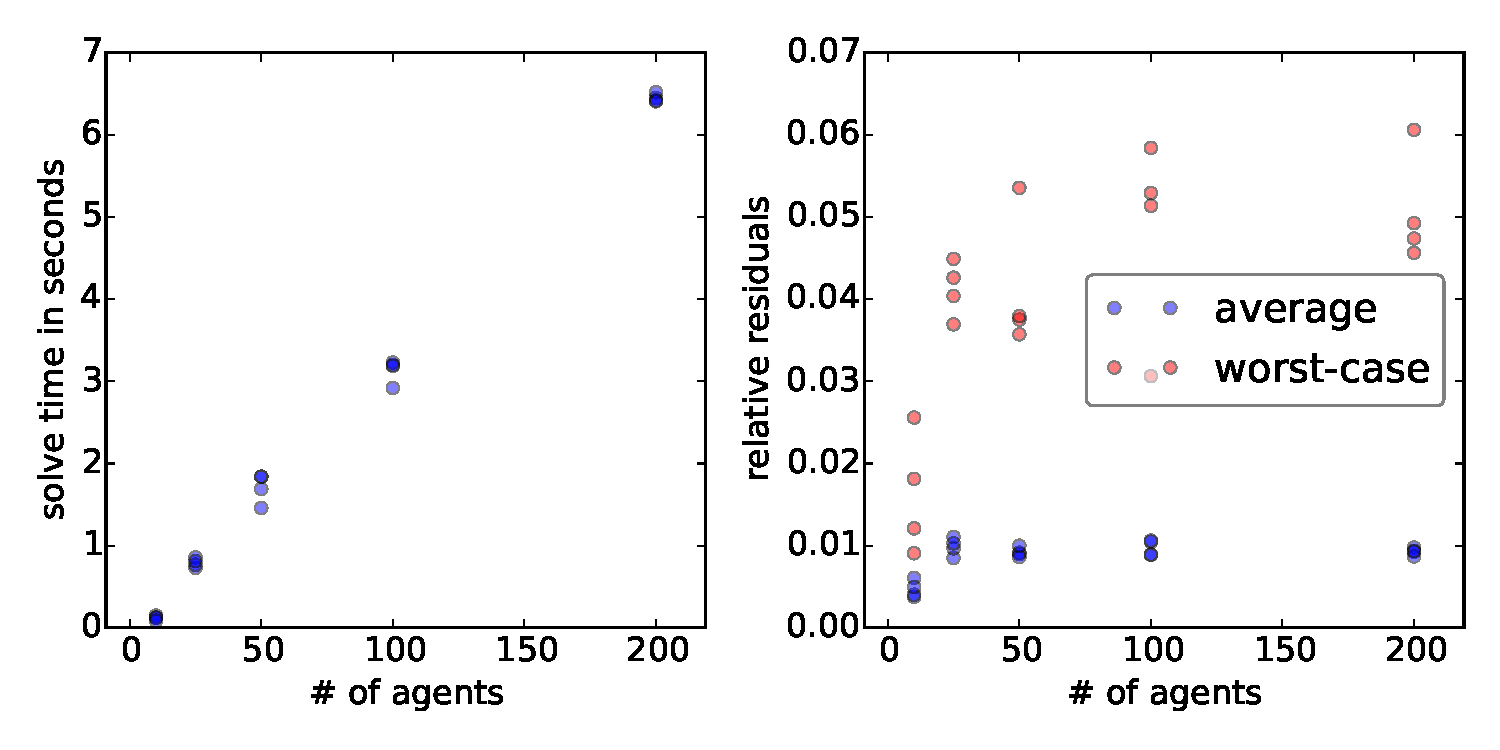
\includegraphics[width=1.0\textwidth]{figures/cvxpy}
\end{center}
\caption{XXX temporary figure. For different values of numbers of agents, $n$,
we generate 10 random instances of a market, as in \S\ref{sec:random_prob}.
We solve each market problem with the centralized method, using SCS, and
report the solve times and average and worst-case relative residuals, with the
statistics taken over the agents in the market, not market instances.}
\label{f-cvxpy}
\end{figure}


\subsection{Decentralized algorithm}

To demonstrate our decentralized algorithm of \S\ref{sec:distributed},
%todo fix section ref
we solve a single random instance of size $n=10^6$ agents. At each iteration,
we take the result of the prox operation (\ref{a-prox}) and the consensus
prices $\Phi^k$ from (\ref{a-phibar}) and compute the average and worst-case
relative residual over the agents in the market and record the findings in
Figure~\ref{f-admm}.

\begin{figure}
\begin{center}
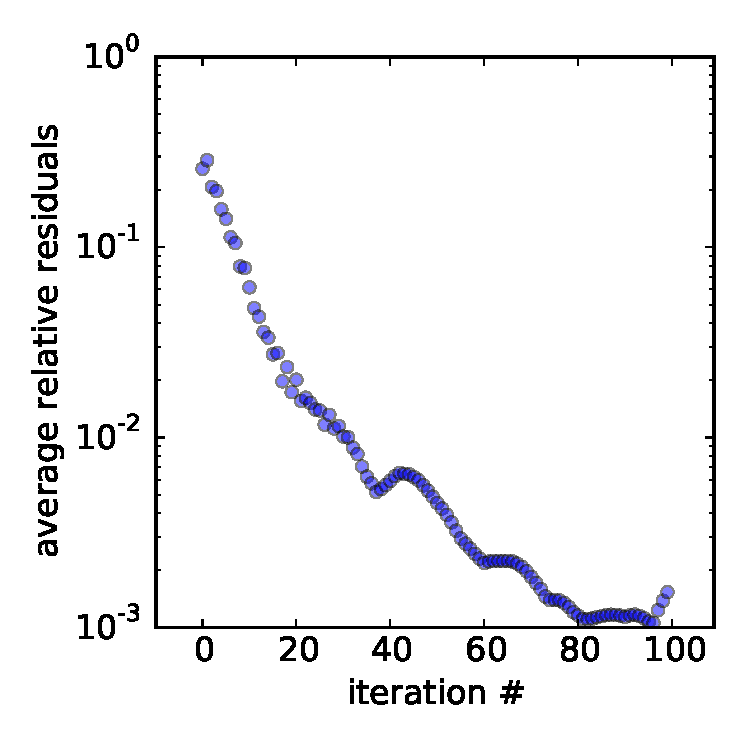
\includegraphics[width=0.6\textwidth]{figures/admm}
\end{center}
\caption{XXX temporary figure. This figure gives results for decentralized ADMM
algorithm applied to a single random market generated as in
\S\ref{sec:random_prob} with $n=10$ agents. We give the average and worst-case
statistics of the agents for their relative residuals.}
\label{f-admm}
\end{figure}


\appendix


\section{Convex optimality conditions for exchange problem}
\label{sec:exchange_proof}

In this section, we use the same definitions and notation as in
\S\ref{sec:exchange_def}.
Consult \cite{BoV:04} as a reference for any
unfamiliar terms in this section.

The exchange UMP~(\ref{p-ump}) for an individual agent has the form
\[
\begin{array}{ll}
\mbox{minimize} & - u_i(x_i)\\
\mbox{subject to} & p^T x_i \leq p^T b_i\\
& x_i \geq 0.
\end{array}
\]

The dual of this problem is
\[
\begin{array}{ll}
\mbox{maximize} & -(- u_i)^*(\tau_i - p y_i) - p^T b_i y_i\\
\mbox{subject to} & y_i \geq 0\\
& \tau_i \geq 0,
\end{array}
\]
with $y_i \in \reals$ and $\tau_i \in \reals^n$. Here, $(- u_i)^*$
is the convex conjugate of the negative utility $-u_i$.

The Karush-Khun-Tucker (KKT) optimality conditions for agent $i$'s UMP consist
of primal feasibility, dual feasibility and zero duality gap. A solution to the
exchange MEP~(\ref{p-mep}) is given by an allocation for each agent which
satisfies that agent's UMP optimality conditions, such that the demand of the
goods does not exceed the supply. Thus, we can write the KKT conditions of the
exchange MEP as
\begin{equation}
\begin{aligned}
p y_i - \nabla u_i(x_i)&= \tau_i\\
y_i p^T x_i &= y_i p^T b_i\\
\tau_i^T x_i &= 0\\
p^T x_i &\leq p^T b_i\\
x_i, y_i, \tau_i &\geq 0\\
\sum_{i=1}^m x_{ij} &\leq \sum_{i=1}^m b_{ij},
\end{aligned}
\label{e-mep-opt1}
\end{equation}
for all $i=1,\ldots,m,\ j=1,\ldots,n$.

We can simplify the constraints by removing $\tau$:
\begin{equation}
\begin{aligned}
p y_i &\geq \nabla u_i(x_i) \\
y_i p^T x_i &= y_i p^T b_i \\
y_i p^T x_i &= \nabla u_i(x_i)^T x_i\\
p^T x_i &\leq p^T b_i\\
x_i, y_i &\geq 0\\
\sum_{i=1}^m x_{ij} &\leq \sum_{i=1}^m b_{ij}.
\end{aligned}
\label{e-mep-opt2}
\end{equation}

Next, the $y$ variables can be eliminated by combining the second and third
constraints in (\ref{e-mep-opt2}) to obtain
\[
y_i = \frac{\nabla u_i(x_i)^T x_i}{p^T b_i},
\]
which we plug it into the first constraint of (\ref{e-mep-opt2}) to get the new
set of constraints
\begin{equation}
\begin{aligned}
\frac{\nabla u_i(x_i)^T x_i}{p^T b_i} p &\geq \nabla u_i(x_i) \\
p^T x_i &\leq p^T b_i\\
x_i &\geq 0\\
\sum_{i=1}^m x_{ij} &\leq \sum_{i=1}^m b_{ij}.
\end{aligned}
\label{e-mep-opt3}
\end{equation}

The second constraint of (\ref{e-mep-opt3}) can be removed, as it is implied by
the others (which we will prove). The resulting set of constraints
\begin{equation}
\begin{aligned}
\nabla u_i(x_i)^T x_i p_j &\geq \nabla_j u_i(x_i) p^T b_i\\
\sum_{i=1}^m x_{ij} &\leq \sum_{i=1}^m b_{ij}\\
p &\geq 0\\
x_i &\geq 0,
\end{aligned}
\label{e-mep-opt4}
\end{equation}
for all $i=1,\ldots,m,\ j=1,\ldots,n$, are equivalent to (\ref{p-exchange-gp}).

\paragraph{Equivalence with original constraints}
We have seen that conditions (\ref{e-mep-opt1}) imply conditions (\ref{e-mep-opt4}).
To see that the opposite implication holds,
multiply $x_{ij}$ with the first inequality of (\ref{e-mep-opt4}) and sum over $j$ to get
\begin{align}
&&\sum_{j=1}^n \nabla u_i(x_i)^T x_i p_j x_{ij} &\geq \sum_{j=1}^n \nabla_j u_i(x_i) x_{ij} p^T b_i \nonumber \\
&\implies & \nabla u_i(x_i)^T x_i p^T x_i &\geq \nabla u_i(x_i)^T x_i p^T b_i \nonumber\\
&\implies & p^T x_i &\geq p^T b_i. \label{e-good-ineq}
\end{align}

We see that
\begin{align*}
\sum_{i=1}^m p^T b_i &\leq \sum_{i=1}^m p^T x_i\ &&\text{(by (\ref{e-good-ineq}))}\\
&= \sum_{j=1}^n p_j \sum_{i=1}^m x_{ij} &&\\
&\leq \sum_{j=1}^n p_j \sum_{i=1}^m b_{ij}\ &&\text{(by second inequality of (\ref{e-mep-opt4}))}\\
&= \sum_{i=1}^m p^T b_i.&&
\end{align*}
This implies equality holds throughout, so, in particular,
\begin{align}
p^T x_i &= p^T b_i \label{e-spending}\\
\sum_{i=1}^m x_{ij} &= \sum_{i=1}^n b_{ij} \label{e-equilibrium}.
\end{align}

This recovers all the constraints from (\ref{e-mep-opt1}), so we see that they
are equivalent to the constraints (\ref{e-mep-opt4}).

We can interpret (\ref{e-spending}) as saying that each agent spends his entire
budget in the equilibrium solution. Constraint (\ref{e-equilibrium}) says that
there are no left-over goods at equilibrium; all goods are consumed.

\newpage
\bibliographystyle{alpha}
\bibliography{bibliography}

\end{document}


